\documentclass[12pt]{article}

\usepackage{fullpage}
\usepackage{graphicx, rotating, booktabs} 
\usepackage{times} 
\usepackage{natbib} 
\usepackage{indentfirst} 
\usepackage{setspace}
\usepackage{grffile} 
\usepackage{hyperref}
\usepackage{adjustbox}
\setcitestyle{aysep{}}


\singlespace
\title{\textbf{Alliance Treaty Design and the Arms-Alliances Tradeoff}}
\author{Joshua Alley\footnote{Graduate Student,
Department of Political Science, Texas A\&M University.}}
\date{{\normalsize \today}}

\bibliographystyle{apsr}

\begin{document}

\maketitle 

\newpage 

\doublespace 

\begin{abstract}

How do differences in alliance treaty design affect military spending by member states? Previous studies of the arms-alliances tradeoff did not address differences in alliance design, leading to mixed empirical support for the proposition that alliance formation leads to reduced military spending. Not all alliances are a good substitute for domestic arms, however. Treaties that obligate alliance partners to fight with few conditions attached are more valuable to members, making them a better substitute for domestic arms. Therefore, unconditional alliance commitments lead to reduced military spending. I test this argument with a multilevel multiple membership model, and find that unconditional alliances are associated with reduced military spending. Comparisons among 314 alliances from 1950 to 2001 suggest that substitution of alliances for arms is uncommon. 

\end{abstract}



\section*{Introduction}

Scholars and policymakers alike believe that international alliances alter military spending by their members. Because arms and alliances provide military capability, these two policies can substitute for each other. Small states can replace their domestic military spending with allied expenditures, so efforts by powerful states to protect their interests through alliances may lead their prot\'eg\'es to reduce military spending. Therefore, accusations of free-riding by junior partners are a staple of alliance politics. 

There are two broad arguments that alliance formation will lead to reductions in defense spending by member states. Theories of the arms-alliances tradeoff emphasizes substitution between arms and alliances \citep{Morrow1993, Sorokin1994}. The economic theory of alliances predicts that small states will reduce defense effort and free-ride on the protection of more powerful partners in their alliance \citep{OlsonZeckhauser1966, SandlerHartley2001}. Although these two theories make a clear prediction, empirical evidence of the association between that alliances membership and defense spending is mixed. Some studies find the expected negative correlation between alliance membership and military spending \citep{Conybeare1992, Sorokin1994, DigiuseppePoast2016}, while others find a positive association \citep{Diehl1994, MorganPalmer2006, QuirozFlores2011}.   

In this paper, I argue that the relationship between alliances and domestic arms depends on the design of the alliance treaty. Non-major powers will only use allied military spending as a replacement for domestic arms when they view the alliance commitment as reliable. Differences in alliance treaty design affect the perceived reliability of an alliance.

States will view treaties that commit partners to fight with few conditions attached as more reliable. Not all alliances guarantee military support, while others attach conditions to intervention, so the association between alliance membership and domestic spending is conditioned by the design of the treaty. In particular, unconditional alliances, which place no conditions on partners' commitments to fight, should lead to reductions in spending. 

I find that unconditional alliances are associated with reductions in military spending by member states. The empirical test uses a multilevel model to captures interactions between alliance-level variation and state-level outcomes. Multilevel modeling strikes a middle ground between detailed studies of dynamics within a few alliances treaties \citep{Reisinger1983, Hansenetal1990, Chenetal1996, PluemperNeumayer2015} and general studies of the association between alliance membership and military spending \citep{Diehl1994, MorganPalmer2006, QuirozFlores2011, DigiuseppePoast2016} by estimating how the characteristics of each alliance modify its effect on member's spending. 

Connecting alliance design and substitution of alliances for arms sharpen our understanding of potential trade-offs in alliance politics. Unconditional treaties provide better deterrence, but the credibility of the alliance allows junior partners to reduce their defense effort. While states may prefer that alliance partners contribute fully to their defense, that goal may be incompatible with credible commitments for deterrence. 

My theory and findings also clarify the extent of substitution. States do not trade alliances for domestic arms as much as the conventional wisdom expects. Instead, substitution is comparatively rare. Given the opportunity to rely on allied capability, small states will take it, but few alliances make substitution possible.   

The next section summarizes and identifies some shortcomings of prior scholarship on the arms-alliances tradeoff. Then I outline a theory of how alliance design and credibility affects state military spending. I then test predictions from that theory using a multilevel multiple membership model, and summarize the results. Last, I conclude with implications for scholarship and policy.  

\section*{Arms versus Alliances}

% Can summarize lit to date here. 

\citet{Altfield1984}, \citet{Morrow1993}, and \citet{MostStarr1989} note that states can use arms or alliances to produce security, making them substitute goods. The economic theory of alliances predicts that smaller allies will ``free-ride'' on the security provided by larger partners \citep{OlsonZeckhauser1966, SandlerHartley2001, Lake2009}. Both theories expect that increasing alliance ties lead reductions in arms spending. 

Another implication of the substitution logic is that states facing economic difficulties will look to alliances for security. \citet{AllenDigiuseppe2013} find that states facing a sovereign debt crisis are more likely to form an alliance to maintain their security while reducing the economic burden of military spending. \citet{Kimball2010} tests whether states with high levels of social demand use substitution and finds a positive correlation between infant mortality rates and alliance formation. 

While the logic of substitution theory is clear, the empirical evidence is mixed. \citet{Diehl1994} and \citet{QuirozFlores2011} find a positive correlation between arms and alliances. \citet{Horowitzetal2017} show that states can use conscription to complement their efforts to form an alliance. \citet{MorganPalmer2006} argue that income effects will lead to increases in arms and alliances, making these complementary goods. Last, \citet{Goldsmith2003} finds no relationship between a dummy indicator of defense pact presence and military expenditures as a share of GDP. 

Research on specific alliances underlines the mixed empirical results from general studies. Most studies of NATO find evidence of free-riding, which has motivated the economic theory of alliances and expectations of substitution more generally \citep{OlsonZeckhauser1966, SandlerForbes1980, Palmer1990, PluemperNeumayer2015, GeorgeSandler2017}.\footnote{The voluminous literature mostly debates the mechanisms and extent of free-riding in NATO. The presence of free-riding is taken as given.} NATO is far and away the best-studied case, but it may not provide generalizable evidence. \citet{Chenetal1996} find little free riding among front-line Arab League members, and there is little free-riding in the Warsaw Pact.\footnote{\citet{ConybeareSandler1990} and \citet{Goldstein1995}  find minimal free-riding in the Triple Alliance and Triple Entente, but the economic theory of alliance would not expect free-riding in those cases.}  

One explanation for these mixed empirical results is that states may only substitute arms for alliances with particular allies. \citet{DigiuseppePoast2016} argue that states are more likely to reduce military spending when they have a democratic ally, whose promises of support are more credible. Democratic allies are not the only possible source of credibility. 

Another source of credibility is the institutional design of the alliance treaty. Alliances make a wide range of promises, which can be more or less valuable. Democracies are also more likely to form limited alliance commitments \citep{Chibaetal2015}, so DiGiuseppe and Poast's results could be an artifact of the kinds of alliances democracies form. To better understand how differences in alliance commitments affect defense effort, I now turn to a theory of alliance design, credibility and state military spending. 


\section*{Theoretical Framework} 

The scope of this theory is limited to junior partners of major power states. These small states have strong incentives to reduce defense effort and ``free ride'' on the protection provided by larger states. By contrast, major powers have less incentive to free ride \citep{OlsonZeckhauser1966}, limiting their ability to trade off between arms and alliances. 

There is one assumption underlying the theory. I assume that states are risk-averse over conflict, due to the consequences of losing a war. The main implication of this assumption is that states will be willing to bear substantial economic and foreign policy costs to maintain their security. 

Following \citet{Morrow1993}, I argue that arms and alliances are imperfect substitute goods. Arms are a more reliable source of military capability, but they take longer to develop than alliances. Alliances provide an immediate capability boost, but they are less reliable than domestic arms. 

In microeconomics, consumption of two goods depends on the marginal rate of substitution and the relative prices of those goods. The basic result in this framework is that individuals will consume as much as possible at the point where their indifference curves are tangential to the budget constraint. This point of tangency occurs when the marginal rate of substitution is equal to the ratio of the prices of these goods. The price ratio depends on the market price of each good, which in this case are the costs of arms and alliances. 

Most theories focus on the relative prices of arms and alliances. As arms become more costly, states are more likely to produce security through alliances \citep{AllenDigiuseppe2013, Kimball2010}. States with high costs of alliances will have more arms and less alliances \citep{Sorokin1994}. Researchers have paid less attention to factors that alter the marginal rate of substitution--- the extent to which alliances can substitute for arms. 

Decreases in the perceived reliability of alliances increase the extent of imperfect substitution between arms and alliances. States can only reduce their defense effort if they believe that the promises of aid during war are credible. Not all alliance treaties are equally credible. 

Alliance treaties contain a wide range of terms, conditions, and obligations for signatories \citep{Benson2011, Chibaetal2015}. The content or institutional design of an alliance treaty affects its credibility. Commitments states make through their alliances have consequences for the credibility of the treaty and subsequent military spending by member states. 

\subsection*{Alliance Design}
% A couple of paragraphs on alliance design considerations

Alliances treaties provide for security cooperation between states. Once some conditions are met, the signatories are obligated to aid their treaty partners in conflict. Treaty design shapes the worth of a treaty by altering the probability of aid, and how much aid signatories can expect. Treaties that promise to join a war with few conditions are more valuable as a source of security. 

The conditions that trigger intervention by partners in an alliance vary widely across treaties. Some pacts are open-ended, requiring engagement after hostilities commence. Other treaties stipulate narrow conditions for intervention, such as the set of belligerents and who started the conflict. The scope of these conditions determines when a treaty has been honored or violated \citep{Leedsetal2000}. 

Beyond the conditions for intervention, not all alliances stipulate a partner must fight. Many alliances only promise consultation with the affected state once the treaty is invoked. These limits on intervention help determine the value of the support to other partners, as participation in the fighting is more valuable. 

In general, alliance treaties must balance between abandonment and entrapment \citep{Snyder1984, Benson2012}. General commitments to fight are highly credible, and reduce partner's fear of abandonment. However, general commitments also come with a risk of entrapment. 

Divergent foreign policy interests create a moral hazard where one alliance partner sets the level of risk, but the other partners bear the costs. Alliance commitments can be used by states to drag treaty partners into conflicts those partners would rather avoid. Greater foreign policy divergence makes states more likely to make limited alliance commitments, out of fear that their partners will entangle them in a war they have no interest in fighting \citep{Benson2012}. 

What are the implications of these differences between alliance treaties for domestic arms? Domestic arms and external alliances are both sources of military capability, but they are imperfect substitutes. Some alliances do not promise enough support, or set broad enough conditions for intervention, to be seen as a reliable source of capability. 



\subsection*{Design and Credible commitments}
% Conditions and promised help determine costs of an alliance in expectation, and therefore its credibility

Domestic arms are a more certain means of offsetting a threat. Direct control of coercive resources makes domestic arms a reliable source of capability for national leaders. By contrast, the capability gains from alliances are more uncertain, as they depend on the credibility of the treaty commitment. As the credibility of an alliance increases, the treaty is seen as more reliable, making it a better substitute for domestic arms. 

What makes an alliance commitment credible? Credible commitments must be costly enough for observers to distinguish them from less meaningful ``cheap talk.'' Alliance treaties derive their credibility from the costs of violation and the expected costs of the promised intervention. 

Violating treaty commitments is costly due to lost reputation \citep{Gibler2008}, spill-overs to other commitments \citep{Crescenzi2012}, and audience costs \citep{Fearon1997, Tomz2007ar, Chibaetal2015, Levyetal2015}. Alliance treaty violation is tied to specific commitments \citep{Leedsetal2000}. Increasing the breadth of the commitments in an alliance, creates more opportunities for violation, increasing the potential cost. 

The expected costs of an intervention depend on the probability of intervention, and the type of intervention a treaty promises. Unconditional commitments increase the probability of intervention, making the treaty for valuable. An unconditional commitment covers the full set of potential conflicts. Conditional commitments address a smaller set of conflicts, so there are cases where partners are not obligated to intervene. 

Promising to join a war is costly in expectation, due to the economic and political demands of war-fighting. Promises of consultation and retaining the freedom to avoid fighting are less costly. Limited commitments allow an alliance partner to hedge its bets by withholding guarantees of full support. To the other members of an alliance, this commitment is not as reassuring.

Consider two hypothetical examples. Alliance A promises consultation under a narrow set of circumstances. So in expectation, the costs of this treaty are low, because it has a low probability of limited support. Alliance B promises to join a war no matter how it started is more costly. Under Alliance B, the signatories agree to pay a higher cost, and make bearing that cost more likely. Alliance B also creates more opportunities for violation, increasing the potential costs of violation. Due its higher expected costs, Alliance B will be seen as more reliable.  

Alliance treaties that only promise support under a narrow set of circumstances, or do not guarantee active military support, are less credible. These alliances are less costly in expectation because they make contingent commitments, or do not promise military engagement. As a result, partner states will view these security commitments as ``cheap talk'' and maintain their defense effort. 

Less credible alliances increase the extent of imperfect substitution with arms by increasing the fear of abandonment. States gain less capability from limited alliances, because they do not expect to receive adequate support. Instead, these states must provide the capability to offset whatever threat they face through military spending. Conversely, more credible promises of support increase the expected capability gains from an alliance, allowing states to substitute treaties for domestic arms spending. 


\subsection*{Predictions}

My theoretical framework generates two testable predictions about the impact of alliance treaty provisions on members' defense spending. Substitution of arms for alliances is obvious when certain alliance characteristics are associated with reduced defense effort. States that maintain or increase spending even after forming an alliance are not free riding. 

General promises of military support will lead to reduced defense effort. Not only are these alliances more credible, but they also cover many potential instances of conflict. Therefore, states can rely on the capability of their allies. Limited commitments that promise little support or make aid less likely will not change national military spending. 

What types of alliances are most likely to reduce defense spending? And which alliance designs will be associated with no change in spending? \citet{Benson2011, Benson2012} divides alliances into unconditional, conditional, pure conditional and probabilistic commitments based on the content of the alliance agreement, which is a useful starting point. 

Probabilistic alliances do not guarantee military support even if the conditions for intervention are triggered. Either through delegation of the final intervention decision to another actor or escape clauses, probabilistic alliances augment uncertainty over whether the alliance partner will intervene. The lack of guaranteed military support especially problematic. Therefore, probabilistic alliances are unlikely to lead to substitution between alliances and arms. Given uncertainty over whether they will receive enough support from their treaty partners, members of probabilistic alliances must maintain their defense effort to hedge against abandonment. 

\begin{quote}
\textsc{Hypothesis 1}: Probabilistic alliances will be associated with no change in defense spending by member states. 
\end{quote}

Unconditional alliances are more credible than probabilistic pacts. In an unconditional alliance, military support does not depend on specific conditions being met. Instead, the partners promise intervention irrespective of how the conflict arose. Unconditional alliances are highly credible, so member states will reduce their defense effort. 

\begin{quote}
\textsc{Hypothesis 2}: Unconditional alliances will be associated with decreases in defense spending by member states. 
\end{quote} 

It is more difficult to make clear predictions about conditional alliances. While these pacts promise military support, their credibility is reduced by the limited breadth of the conditions. The scope of the conditions that trigger intervention also varies widely across treaties. The most important concern for states seeking security from an external threat is whether their alliance covers the most important threats. Absent more detail on the exact conditions of an alliance and key threats to members, it is hard to make predictions. Still the ambiguity in these treaties mean their expected impact on spending should be close to zero.

Many alliances have none of Benson's key characteristics. These treaties promise only consultation, or a mix of consultation and non-aggression. Such limited commitments should have no effect on spending. This makes these alliances that promise no aid a natural comparison category for testing the impact of probabilistic and unconditional alliances on military spending. 

\subsection*{Limitations} 

The above theory has two limitations. Alliance designs are highly strategic. The characteristics of partner states determine whether they form an alliance and how those treaties are designed. Because they face higher audience costs for reneging on their commitments, democracies are more likely to form alliances that only obligate them to consult with a partner, or specify limits to their defensive obligations \citep{Chibaetal2015}. Shared interest and the level of threat faced by a client state may explain why some clients get unconditional defense pacts \citep{Yarhi-Miloetal2016}. At the moment, I control for some correlates of the formation process, but do not address it in theoretical or empirical detail.

A theoretical narrative that produces the opposite prediction of my framework emphasizes the role of regime type. If democracies are more likely to form alliances that only obligate them to consult with partners, or limit their commitments, but are generally reliable partners \citep{Chibaetal2015, DigiuseppePoast2016}, then even limited commitments might lead to reduced defense effort. This alternative requires that the high credibility of the limited commitments outweighs the constrained support, and can be controlled for in an empirical analysis. Including democracy and alliance design considerations in the same model will likely provide a better picture of the effect each variable has on defense effort. 

The scope conditions are another limitation. The dynamics I describe above apply primarily to smaller states, not to major powers. Major powers have a fundamentally different set of foreign policy concerns. It is possible that the same associations between alliance design and major power military spending apply only to alliances between major powers. In the interest of theoretical and empirical parsimony, I focus on non-major powers only. 

Careful empirical design is necessary to accurately estimate the relationship between alliance characteristics and defense spending. Attention to the structure of alliance data is perhaps the most important concern, and control variables can account for many of the strategic concerns around alliance designs In the next section, I describe my research design. 
 

\section*{Research Design} 

I test my two hypotheses on 159 non-major powers in the international system from 1950-2001, which includes all states besides the Correlates of War project's list of major powers.\footnote{China, France, Russia, the UK, US as well as Japan and Germany after 1990 are the major powers I removed from the sample.} While this sample has limited temporal coverage, it ensures my results are comparable to work by \citet{DigiuseppePoast2016} and \citet{Nordhausetal2012}.\footnote{These researchers limit their samples based on the quality of key economic indicators.} Using the same sample is especially helpful for comparison because I use a different estimator from other studies of the relationship between arms and alliances. 

Most studies of the arms-alliances tradeoff estimate regression models on state-year panel data. Researchers use averages or dummy variables to summarize key characteristics of each state's alliance portfolio. For example, \citet{Benson2012} uses a dummy variable to indicate if the state that initiated a militarized interstate dispute (MID) had a conditional alliance. \citet{DigiuseppePoast2016} use a dummy indicator of whether a state has at least one defensive alliance tie with a democratic state. This approach limits our ability to compare individual alliances and generate the risk that arbitrary data transformations are driving the results \citep{GelmanLoken2013}. 

Averaging or the use of dummy variables at the state-year level eliminates important variation between alliances. Without an explicit model of between alliance variation, there may be too much certainty in alliance parameter estimates \citep{McElreath2016} because state level measures reduce the amount of variation in alliance-level variables. In the post-war period, many states are members of alliances like NATO and Rio Pact for the entire sample- so there is limited within-state variation in many dummy indicators. 

The standard modeling approach is especially problematic for my theory, which emphasizes differences in \textit{alliance-level} characteristics. Modeling alliance-level variation can better control for multiple characteristics of alliances, especially correlates of alliance design and state spending that might otherwise lead to omitted variable bias. The usual single-level cannot make direct comparisons between alliances as institutions, which is essential to testing my theory. 

Therefore, I use a multiple membership multilevel regression model, which models variation among observations clustered within alliances, states and years. Multilevel modeling allows me to directly estimate the impact of alliance-level covariates on state-level outcomes \citep{GelmanHill2007}. I can also use the model make detailed comparisons between alliances to test secondary implications of the theory. 

Multilevel models account for sampling imbalance between groups by pooling strength and shrinking estimates towards an overall average. Partial pooling approach leads to estimates of the amount of variation between alliances and states, avoiding maximal overfitting or underfitting. Borrowing strength and shrinkage allows for plausible estimates of the effect of alliances with limited variation in membership over the sample. 

Using a multilevel model has costs. Defining a separate regression for each level of the data requires additional assumptions about the distributions characterizing of state and alliance clusters \citep{McElreath2016}. Also, these models are computationally intensive and more difficult to estimate.

Hierarchical models are the most well-known type of multilevel model, where units are nested inside one another. State membership in alliances is less neat--- many states are members of multiple alliance treaties, and different states are clustered within each treaty. Such multiple-membership data requires a different model. 

My model predicts annual military spending by non-major power states using state and year varying intercepts, state-level variables, and the weighted sum of spending by other states in its alliances. Alliance characteristics predict the importance of spending by the other members of a particular treaty for spending by each member. Therefore, I directly link a wide range of alliance treaty characteristics and military spending. 

\subsection*{Model Details}

Varying intercept parameters encode the different clusters of observations in a multilevel model. These parameters are essential to modeling variance among groups within the data. Varying intercepts allow partial pooling among observations, which reduces the risk of maximally over or underfitting the data. I include an overall intercept parameter along with random intercepts for each year and states. The varying intercepts capture state and year specific deviations from the overall mean.

The dependent variable has a mean and median of 6.7, and half the observations fall between 5.2 and 8.2. The data itself has heavy tails, as some larger countries spend a great deal in a given year, and smaller states spend very little. The largest and smallest values are more than 3 standard deviations away from the mean, and there are more observations in the tails than a standard normal distribution. To ensure that the distribution of the outcome places adequate weight in the tails, I use a student's t distribution \citep{JuarezSteele2010}.\footnote{Fitting the model with a normally distributed outcome leads to poor performance for LOO and WAIC model comparison, which is further evidence that a a robust model is necessary \citep{Vehtarietal2017}}  The degrees of freedom parameter $\nu$ is estimated from the data using a gamma prior.

Formally, the full model can be expressed as follows, starting with state-year changes in the natural log of military spending $y_{it}$:
\begin{equation}
y_{it} \sim student_t(\nu, \mu, \sigma) 
\end{equation}

The mean of this distribution $\mu$ is a linear function of the overall mean $\alpha$, state varying intercepts $\alpha^{st}$, year varying intercepts $\alpha^{yr}$, a lagged dependent variable $\eta y_{t-1}$, and a matrix of state-level regressors $W_{it}$ with a vector of parameters $\gamma$. The impact of alliance membership on military spending is the weighted sum of allied capabilities. The alliance-level variables predict the weight of each alliance. 

In the model, I connect alliance membership and military spending by multiplying a column vector of alliance weights by a row vector of state $i$'s alliance memberships at time $t$ $Z_{it}$. The columns of $Z$ correspond to individual alliances, marked by their ATOP id. Each element of $Z_{it}$ is equal to the total log-transformed military spending of all other states in an alliance if a state is a member of an alliance in a given year. All other elements of the membership matrix $Z$ are zero. The non-zero values are rescaled by two standard deviations to facilitate model fitting.\footnote{Having parameters with different scales creates large differences in posterior variance, which makes posterior sampling more difficult.} 

Using alliance spending means that membership in different alliances is not treated equally. By multiplying the membership matrix $Z$ by the vector of weights $\lambda$, the impact of a state's alliances on spending is a weighted sum of spending by other members of its alliances. This specification tweaks a classic ``aggregation technology'' from the economic theory of alliances, where potential free riding depends on the sum of allied spending \citep{Murdoch1995}. A weighted sum leverages my theory that the impact of allied capability of spending depends on the promises those allies made. The full state-level model is:

\begin{equation}
\mu_{it} = \alpha + \alpha^{st} + \alpha^{yr} + \eta y_{t-1} + W_{it} \gamma + Z_{it} \lambda 
\end{equation}

I assume that each alliance weight $\lambda_k$ is normally distributed, with mean $\theta_k$ and variance $\sigma^{all}$. $\theta_k$ is predicted by a second-level regression using the alliance characteristics. Therefore:

\begin{equation}
\lambda_k \sim N(\theta_k , \sigma^{all})
\end{equation} 
and 
\begin{equation}
\theta = X \beta
\end{equation}

The regressors in the alliance-level model predict how states weight an alliance's spending in setting their own military expenditure. Because my theory addresses the impact of alliance design on military spending, the $\beta$ parameters are the primary quantity of interest. A negative $\beta$ implies that a particular alliance variable decreases $\lambda$ and by extension, military spending.

The state-level variables $W_{it}$ control for state characteristics that also affect military spending and may be correlated with alliance design. Without controlling for differences between states, we might over-estimate the importance of alliances. The lagged dependent variable accounts for serial correlation, and changes the interpretation of the model, allowing me to calculate the long-run impact of different variables. 

Consider one observation from Argentina as an example of how the model works. Argentine military spending in 1955 depends on Argentina's GDP, regime type, and other variables, as well as varying intercepts for Argentina and 1955. In 1955, Argentina was a member of two alliances- the Rio Pact and the Organization of American States (OAS). So Argentina's spending in 1955 was also a function of the total spending of all other Rio Pact and OAS members, weighted by the credibility of those treaties. The model predicts a $\lambda$ parameter for the OAS and Rio Pact based on the institutional features of those two treaties--- the Rio Pact is probabilistic deterrent, while the OAS is a conditional deterrent pact. 

\subsection*{Variables} 

The dependent variable is the log-transformed value of a state's military expenditures during each year. I also included a lag of the dependent variable, so that the model is equivalent to estimating changes in expenditure \cite{DeBoefKeele2008}. Using a lagged DV also allows direct estimates of the speed and extent of adjustments in spending. Expenditures change slowly over time, and I am estimating a partial adjustment model that implies changes in the independent variables will start an adjustment process that ends in a new equilibrium, ceteris paribus. Estimating changes directly imposes the assumption that unconditional alliances lead to negative changes as long as they are active, which is difficult to justify. 

Military expenditure is the most common proxy for defense effort. Following \citet{DigiuseppePoast2016} I use spending data from \citet{Nordhausetal2012} who combine data from the Stockholm International Peace Institute (SIPRI) and Correlates of War (COW) projects to address defects in each.\footnote{SIPRI tends to under report spending by Warsaw Pact nations during the Cold War, while the COW data has some instances of measurement error.} The log transformation ensures the data are closer to normally distributed, but even then a robust regression is necessary. 

I draw on two databases for measures key alliance characteristics. To test Hypotheses 1 and 2, I use the alliance classification of \citet{Benson2012}. In my sample, there are 314 total alliances. Each alliance has a dummy variable indicating whether it is a conditional, unconditional, probabilistic deterrent, or compellent treaty, and alliance can fall into multiple categories. There are 38 unconditional, 30 probabilistic, and 80 conditional deterrent alliances. All 12 compellent alliances are unconditional and also have unconditional deterrent conditions. 179 alliances do not have any of Benson's conditions. All data on state membership in alliances comes from the ATOP project \citep{Leedsetal2002}. 

Controlling for some other types of alliances changes the interpretation of the key independent variables by altering the comparison category for each binary variable. While testing the impact of probabilistic and unconditional alliances, I control for whether an alliance has compellent aims and conditional deterrent alliances. Therefore, the remaining 179 alliances that promise consultation are the base category. Following previous work, I remove non-aggression pacts from the alliance sample, so these alliances are mainly pacts that promise only consultation, or both consultation and non-aggression. 

Accounting for state and alliance characteristics that may be correlated with both alliance design and military expenditures is necessary to avoid omitted variable bias in the estimates. At the alliance level, I include binary indicators of whether an alliance stipulates military aid, and if any member was involved in a war when the alliance was formed \citep{Leedsetal2002}. I also include the average democracy of the alliance members at the time of formation, because democratic membership is associated with alliance design \citep{Chibaetal2015} and spending by member states \citep{DigiuseppePoast2016}. I also control for the number of alliance members at the time of formation. Last, I control for superpower support with dummy indicators of whether the US or Russia were members of the alliance.  

The first set of state-level controls addresses the geopolitical environment for each state. Dummy indicators of participation in international war or civil war capture conflict participation, which can make defense a superior good \citep{OlsonZeckhauser1966}. I also include the military expenditures of rival states and a dummy variable indicator of Cold War years in the sample to measure potential arms competition. The natural log of GDP, and the POLITY measure of political institutions control for key domestic characteristics \citep{FordhamWalker2005}. GDP, POLITY, and rival military expenditures are all re-scaled by two standard deviations for ease of estimation and interpretation. 


\subsection*{Estimation and Priors} 

I estimate the model in \textsf{R} using STAN \citep{Carpenteretal2016}. STAN is a probabilistic programming language that supports full Bayesian inference, approximating the posterior distribution using Hamiltonian Monte Carlo (HMC). Clarity about the prior distributions is essential when fitting a multilevel regression model in the Bayesian framework. I have some information about the most likely coefficient values based on the scale of the dependent variable and the use of rescaled regressors, so weakly informative priors are appropriate \citep{Gelmanetal2014}. 

The range of plausible coefficient values can be captured without using heavy-tailed priors, so I use normally distributed priors with a mean of zero and standard deviation of one for the regression coefficients. Using heavier-tailed priors such as the Cauchy distribution on the coefficients in place of the normal priors is much more computationally expensive and can lead to nonsensical posterior predictions. Furthermore, the normal prior places 95\% of the prior weight on coefficient values between negative two and two, which does not rule out some large coefficients relative to the scale of the dependent variable. 

\autoref{tab:priors} summarizes all the prior distributions from the model. The estimated mean $\alpha$ is different from the mean of the data due to the inclusion of the lagged dependent variable. A normal prior with mean zero and standard deviation of three is diffuse enough to capture the sample mean and a wide range of other values besides that. 

I place half-normal priors with mean zero and a standard deviation of one on the variance hyperparameters in the model. Given the scale of the data, these priors are diffuse enough to allow for a wide range of pooling among states, years, and alliances. Larger estimates of the variance parameters imply that complete pooling assumptions for the different groups are inappropriate. Fixed effects models assume no pooling of groups and impose an infinite estimate on the variance hyperparameters. 

The small scale on the gamma prior for the degrees of freedom parameter $\nu$ makes the prior diffuse enough to allow many possible distributions \citep{JuarezSteele2010}. As the degrees of freedom in a t-distribution decreases, more probability mass shifts out into the tails. A t-distribution with infinite degrees of freedom is equivalent to a normal distribution, on one hand, while the same distribution with one degree of freedom is equivalent to a Cauchy distribution. To avoid excessive posterior mass in the tails, and posterior predictions that far exceed the range of the observed data, I place a lower bound at four on the $\nu$ parameter. 


\begin{table} % Create a table of priors.

 \begin{center}
\begin{tabular}{c} 
$ p(\alpha) \sim N(0, 3)$  \\
$ p(\sigma) \sim \mbox{half-}N(0, 1) $ \\
$ p(\alpha^{yr}) \sim N(0, \sigma^{yr}) $ \\ 
$ p(\sigma^{yr}) \sim N(0, 1) $ \\
$ p(\alpha^{st}) \sim N(0, \sigma^{st}) $ \\ 
$ p(\sigma^{st}) \sim \mbox{half-}N(0, 1) $ \\ 
$ p(\sigma^{all}) \sim \mbox{half-}N(0, 1) $ \\
$ p(\eta) \sim \mbox{half-}N(0, 1) $ \\
$ p(\beta) \sim N(0, 1) $ \\
$ p(\gamma) \sim N(0, 1) $ \\ 
$ p(\nu) \sim gamma(2, 0.1)$ 
\end{tabular} 
\end{center} 

\caption{Summary of Priors for Multilevel Model}
\label{tab:priors}
\end{table} 

A major limitation of this model is that it does not account for time-varying alliance characteristics. Future work can address this issue. My theoretical focus on alliance design makes the focus on time-invariant characteristics acceptable for the moment- treaty conditions do not change over time without the alliance indicator changing in the ATOP data. Using spending by other members in the alliance membership matrix captures changes in the capability of the alliance over time, which would otherwise be a key omitted variable. 

There are 314 alliances in the sample, each with its own $\lambda$ parameter. In addition, all 49 years and 159 states have their own intercept. To facilitate estimation, I use a non-centered parameterization for the intercepts,\footnote{Also known as a standardized adaptive prior} which separates the hierarchical parameters out from lower-level model parameters \citep{McElreath2016}. The mean and variance of the intercept parameters are strongly correlated, which makes sampling from the posterior more difficult \citep{BetancourtGirolani2015}. Non-centered parameterization is another way of expressing the same model to improve sampling and protect the validity of inferences. 


\section*{Results} 

All the results are based on four chains which take 2,000 samples from the posterior distribution after a warm-up of 1,000 samples. All standard diagnostic tests indicate that the chains converged. There is adequate mixing in the chains, no divergent iterations, and the $\hat{R}$ statistic is well below 1.1 for all parameters.\footnote{See the appendix for more detail on these diagnostics.} I also validate the model fit using posterior predictive checking. 

Because of the log-transformed dependent variable, the regression coefficients are partial elasticities. There is some empirical support for my expectations. Unconditional pacts are associated with decreased military spending, while probabilistic deterrent and conditional deterrent pacts have no impact on spending. \autoref{fig:post-prob} plots the posterior probability each regression coefficient is positive. 

\begin{figure}[htbp]
	\centering
  \includegraphics[width=0.95\textwidth]{C:/Users/jkalley14/Dropbox/Research/arms-allies/figures/post-prob.png}
	%\includegraphics[width=0.95\textwidth]{C:/Users/Josh/Dropbox/Research/arms-allies/figures/post-prob.png}
	\caption{Posterior Probability each model coefficients is positive. Precise posterior probability at the end of each bar.}
	\label{fig:post-prob}
\end{figure}


There is only a 93.6\% chance that conditional alliances are associated with decreased spending. Probabilistic deterrent and conditional deterrent pacts have 25\% and 28\% positive posterior probability, respectively. Only the effect of conditional deterrent pacts can be reliably distinguished from zero, if we use the standard 90\% cutoff for Bayesian posterior probabilities.\footnote{I use a 90\% threshold because 95\% estimates can be unstable.}

Among the other alliance-level variables, the wartime alliance coefficient has over 90\% positive posterior probability. A two-standard deviation change in the share of democratic members in an alliance at the time of formation is associated with decreased spending by member states, as 91.8\% of the posterior mass falls on negative values. Institutionalization nearly meets the 90\% threshold as well, which suggests formal institutions might provide a check on free-riding. 

Most state-level covariates are associated with increases in spending, especially international and civil war. A two-standard deviation change in a state's POLITY score is correlated with reductions in spending. Cold war years and higher GDP are also associated with increased spending.

The data-generating process for military spending is highly autoregressive. The posterior mean of the lagged DV coefficient is .97, and while the posterior density does not include one, the coefficient is large enough to suggest that military expenditures are non-stationary for most states. Nearly integrated time series have many similar properties to non-stationary series \citep{DeBoefGranato1997}, so including the lagged DV to account for autocorrelation is essential. 

The distribution of the alliance weight parameters $\lambda$ provides additional evidence for the negative association between unconditional alliances and military spending. \autoref{fig:lambda-box} summarizes the posterior mean of the $\lambda$ parameter for each alliance. 36 of the 38 unconditional alliances have a negative mean $\lambda$.  

\begin{figure}[htbp]
	\centering
		\includegraphics[width=0.95\textwidth]{C:/Users/jkalley14/Dropbox/Research/arms-allies/figures/lambda-box.png}
		%\includegraphics[width=0.95\textwidth]{C:/Users/Josh/Dropbox/Research/arms-allies/figures/lambda-box.png}
	\caption{Distribution of Posterior mean alliance weights divided by military spending. Circles indicate multilateral alliances, and the size of the circle corresponds to the number of members.}
	\label{fig:lambda-box}
\end{figure}

For most treaties with none of Benson's conditions, the posterior mean of $\lambda$ is near zero. Conditional deterrent alliances have a similar distribution, albeit with more positive $\lambda$ values in multilateral treaties. There is a wider range to the weights for probabilistic deterrent alliances, which likely reflects that 12 of those treaties were formed by the United States, which has substantial military spending for allies to free ride on. 

What is the substantive importance of unconditional deterrent alliances for military spending? Given the autocorrelated data-generating process, the long-run multiplier of unconditional deterrent pacts is equal to $\frac{\beta_{uncond}}{ 1 - \eta}$. This can be calculated for each draw from the posterior, resulting in a full posterior distribution of the long-run effect. 

The posterior mean of the long-run multiplier for an unconditional deterrent pact is $-0.75$. Because posterior of the lagged DV coefficient is entirely positive, the posterior probability that the long-run multiplier is negative is the same as the unconditional alliance coefficient; $.934$. The long-run effect of an unconditional alliance is similar to the impact of a two-standard deviation change in a state's POLITY score.

\autoref{fig:non-zero alliances} plots posterior mean of the $\lambda$ parameters for those alliances where there is more 90\% of the posterior mass of the weight parameter $\lambda$ is positive or negative. There are 19 such alliances. Eight alliances have positive association with military spending, including the Arab League (ATOP ID 3015) and a 1993 alliance between Georgia and Azerbaijain (ATOP ID 4425). In interpreting this plot, recall that the weight parameters depend on all the alliance covariates, not just the type of commitment. 

Among the eleven alliances with a robust negative weight for member's military spending, four are unconditional treaties, and six are probabilistic deterrent pacts. NATO (ATOP ID 3180) is the only conditional deterrent alliance with a discernible negative effect on member's military expenditure.  The Rio Pact (ATOP ID 3075) is a noteable probabilistic deterrent pact that is associated with reduced spending, which does not match my theoretical predictions. This may reflect the breadth of the treaty, which included most Latin American states. Coupled with US hegemony in Latin America, the Rio Pact diminished regional arms competition. NATO and the Rio Pact are common examples of substitution, so these predictions add face validity to the results. 

The other five probabilistic deterrent pacts that have a clear negative weight are bilateral treaties between the United States and Asian or Middle Eastern states. While the negative weights for these six alliances are not predicted by my theory, these results reflect the combination of strong security fears and American capability. From 1950 to 2001, the US formed one unconditional, four conditional deterrent, and twelve probabilistic deterrent alliances. Given the kinds of alliances the US formed, a probabilistic commitment was a meaningful signal of US support. 

\begin{figure}[htbp]
	\centering
		\includegraphics[width=0.95\textwidth]{C:/Users/jkalley14/Dropbox/Research/arms-allies/figures/non-zero alliances.png}
		%\includegraphics[width=0.95\textwidth]{C:/Users/Josh/Dropbox/Research/arms-allies/figures/non-zero alliances.png}
	\caption{Posterior mean of the weight parameter $\lambda$ for alliances with better than a 90\% chance of being positive or negative. The number attached to each column summarizes the exact posterior mean. Bars are colored by alliance type.}
	\label{fig:non-zero alliances}
\end{figure}

The three smallest posterior means are unconditional treaties, including a 1981 Israel-US treaty (ATOP ID 3925), a 1981 treaty between Gambia and Senegal (ATOP ID 3930),  and the 1956 alliance between France, Israel and the UK (ATOP ID 3322). The other unconditional treaty that led to reductions in arms spending is a 1960 treaty between the UK, Greece, Turkey and Cyprus (ATOP ID 3405). 


\subsection*{Model Performance and Comparison}

Adding alliance membership and predicting the weights makes my model of military spending much more complicated. Does that complexity improve model fit? I used leave-one-out cross validation (LOO) \citep{Vehtarietal2017} and \citet{Watanabe2010}'s Widely Applicable Information Criteria (WAIC) to compare the full model with a specification that includes only the varying intercepts and state-level variables. Both these methods estimate out-of-sample prediction accuracy using simulations of the log-likelihood. 

There is no significant difference in LOO between the state and full models. While the full model has a smaller WAIC and LOO values, the difference in LOO is not statistically significant. Given the added complexity of the alliance model, the lack of improvement is not surprising. I retain the alliance model because it offers a direct test of theory without losing predictive accuracy. 

The partial pooling of the multilevel model is especially helpful in this data, because the within-group variance of years, states, and alliances is not the same. Much of the posterior mass for the alliance variance hyperparameter is concentrated near zero, implying extensive pooling of alliances. There is a 93\% chance that variance among states is larger than variance among alliances. Furthermore, there is a 95\% chance that variance among years is larger than variance among states. The full posterior densities of the variance hyperparameters are shown in \autoref{fig:variance-hyperparam-plot}. 

\begin{figure}[htbp]
	\centering
		\includegraphics[width=0.95\textwidth]{C:/Users/jkalley14/Dropbox/Research/arms-allies/figures/variance-hyperparam-plot.png}
		%\includegraphics[width=0.95\textwidth]{C:/Users/Josh/Dropbox/Research/arms-allies/figures/variance-hyperparam-plot.png}
	\caption{Posterior density of the variance hyperparameters. Each hyperparameter is an estimated of the variance among states, years and alliances in the data.}
	\label{fig:variance-hyperparam-plot}
\end{figure}


\section*{Discussion} 

Most of the results correspond with my prediction that more credible alliance treaties lead to reductions in military spending. Unconditional alliances are associated with reductions in military spending. Less credible commitments such as probabilistic deterrent alliances have no impact on military spending. 

Some probabilistic deterrent alliances do lead to reductions in defense effort. Understanding what makes these treaties credible despite limited and contingent promises of support is an important task. Shared interests is one possible explanation--- when states are closely aligned, the exact content of an agreement is less important than the existence of a formal agreement. 

Another matter I do not address is how threat might modify the relationship between alliance conditions and spending. The probabilistic deterrent pacts that led to reductions in spending were treaties between the US and states in intense security competition, including Pakistan, Turkey, and Taiwan. Under these conditions, a superpower commitment provides some assurance, which leads states to reduce spending from a high base. 

My finding that alliances with more democratic members at the time of formation are associated with reduced spending corroborates the work of \citet{DigiuseppePoast2016}. These results should still be treated with caution, because I only measure the proportion of democracies at the time of formation. The democratic composition of alliances often changes over time \citep{GiblerWolford2006}, but my model does not account for that. 

With these alliance comparisons in hand, what judgments can we make about theories that predict substitution between arms and alliances? Substitution between arms and alliances is uncommon. Most alliances do not offer enough capability or credible promises to change the military expenditure of member states. 

Of the 314 alliances in this sample, only 19 have a clear cumulative impact on spending, even if particular characteristics do. States that form an alliance usually continue spending as if that treaty did not exist. The logic of free-riding is sound, but most individual treaties have little free riding.

Furthermore eight of those 19 treaties are associated with increased spending, which implies arms and allies are complements in those cases. Two of the eight alliances (ATOP IDs 4425 \& 4535) involved Azerbaijan during their 1993 war with Armenia. The Arab League (ATOP ID 3015) is another alliance that was associated with increased defense effort, as members faced substantial conflict risks with Israel. In the right context, alliances can be complements to arms. 

Although substitution is rare, it is important. NATO and the Rio Pact are cornerstones of contemporary geopolitics. South Korea's alliance with the United States is pivotal to East Asian security. 

The focus on the arms-alliances tradeoff and substitution in academic theory may be a consequence of the empirical and theoretical emphasis on NATO. Due to data availability and policy relevance, there are many studies of free-riding by NATO members. But NATO is unusual--- no other conditional deterrent treaty is associated with substitution. Understanding NATO is valuable, but that emphasis may inflate our sense of how common substitution is. 

Previous mixed empirical results in tests of the substitution hypothesis likely reflect changes in model specification and the sample which give more or less weight to different treaties. A small subset of alliances lead to substitution, and the extent of cross-sectional and temporal variation in membership of those and other treaties will shift with small changes in empirical strategy. My findings suggest that alliances can be substitutes or complements for arms, and the relationship depends on the characteristics of the alliance. 

My focus on comparing individual alliances does not address the cumulative impact of a state's alliance portfolio. The total weighted sum of allied spending may encourage free-riding where individual free-riding. A refinement of the the theory and another set of calculations could address this issue.  

Another possible limitation of the above results is non-random alliance design. I attempt to address this problem in the design by controlling for things like the share of democratic members at the time of formation, regime type, and alliance institutionalization. While I believe that the set of control variables is comprehensive, this solution may still be incomplete. 



\section*{Conclusion}

In this paper, I argue that unconditional alliances are more likely to result in substitution away from arms by member states, because these treaties are more credible. By contrast, probabilistic deterrent pacts are less credible, and do not lead to changes in expenditure. Using a statistical model connecting differences in alliances with member's military spending, I found some empirical support for these predictions.

The multiple membership multilevel model I apply here could be useful for other social scientists. Multiple international organizations simultaneously affect state-level outcomes from human rights treaties to trade and foreign investment. Instead of selecting a few key organizations, or using state-level averages, scholars could use this model to compare the impact of multiple organizations and their characteristics. 

This paper leaves several open questions for future research on the arms-alliances tradeoff. The evidence I presented here could be unique to the post-World War II period. Expanding the sample would introduce more variation between the different types of alliances, as well as add substantial measurement error in the dependent variable and key controls, especially GDP. Future work should consider a wider sample, to test the generalizability of my findings. Modeling the design and consequences of alliances simultaneously may be another worthwhile empirical task. 

How alliance design affects the composition of state spending is another open question. In alliances where substitution occurs, what do free-riders spend their gains on? Do states alter their force structure by forgoing expensive weapons systems? 

The theory and results of this paper are relevant for policy. If policymakers want to dampen arms competition, unconditional alliances can provide credible assurances, but the free-riding may also increase. The goals of deterrence through credible assurances and avoiding free-riding by junior partners are in tension. Any potential spending reductions must also account for moral hazard \citep{Benson2012}. 

We should be careful about generalizing lessons from NATO to other alliances. NATO is an excellent example of substitution and free-riding, but it is an unusual institution. No other conditional deterrent pact leads to reductions in military spending by member states. NATO's regional scope, institutionalization, and US involvement make it a uniquely influential alliance and difficult to generalize from. 

My results suggest that fear of abandonment can lead states to increase military spending. So President Trump's suggestions that the US may not support allies that fail to meet NATO's 2\% military spending obligation may have the desired effect of increasing spending. Less credible commitments have other costs such as inviting external aggression, and my findings cannot adjudicate between those costs and benefits. A myopic focus on free-riding, which is relatively rare, has other foreign policy costs. 

Understanding differences in alliance design helps resolve an outstanding empirical puzzle in international relations research. Previous mixed empirical results reflect a lack of attention to alliance design. Unconditional alliances are one of the main drivers of substitution between arms and alliances. As states design new security institutions, they must balance the need for deterrence from credible promises, moral hazard, and the potential for free-riding. Althought substitution of alliances for arms is uncommon, this paper helps us understand when it is most likely. 






\bibliography{C:/Users/jkalley14/Dropbox/Research/MasterBibliography}  
%\bibliography{C:/Users/Josh/Dropbox/Research/MasterBibliography} 





\end{document}
